%%
%% This is file `tikzposter-template.tex',
%% generated with the docstrip utility.
%%
%% The original source files were:
%%
%% tikzposter.dtx  (with options: `tikzposter-template.tex')
%%
%% This is a generated file.
%%
%% Copyright (C) 2014 by Pascal Richter, Elena Botoeva, Richard Barnard, and Dirk Surmann
%%
%% This file may be distributed and/or modified under the
%% conditions of the LaTeX Project Public License, either
%% version 2.0 of this license or (at your option) any later
%% version. The latest version of this license is in:
%%
%% http://www.latex-project.org/lppl.txt
%%
%% and version 2.0 or later is part of all distributions of
%% LaTeX version 2013/12/01 or later.
%%


\documentclass{tikzposter} %Options for format can be included here

\usepackage{todonotes}

\usepackage[tikz]{bclogo}
\usepackage{lipsum}
\usepackage{amsmath}

\usepackage{booktabs}
\usepackage{longtable}
\usepackage[absolute]{textpos}
\usepackage[it]{subfigure}
\usepackage{graphicx}
\usepackage{cmbright}
%\usepackage[default]{cantarell}
%\usepackage{avant}
%\usepackage[math]{iwona}
\usepackage[math]{kurier}
\usepackage[T1]{fontenc}


%% add your packages here
\usepackage{hyperref}
% for random text
\usepackage{lipsum}
\usepackage[english]{babel}
\usepackage[pangram]{blindtext}

\colorlet{backgroundcolor}{blue!10}

 % Title, Author, Institute
\title{New York City Taxi Trip Duration}
\author{Siyi Yu$^1$}
\institute{$^1$ Jilin University, China \\
}
%\titlegraphic{logos/tulip-logo.eps}

%Choose Layout
\usetheme{Wave}

%\definebackgroundstyle{samplebackgroundstyle}{
%\draw[inner sep=0pt, line width=0pt, color=red, fill=backgroundcolor!30!black]
%(bottomleft) rectangle (topright);
%}
%
%\colorlet{backgroundcolor}{blue!10}

\begin{document}


\colorlet{blocktitlebgcolor}{blue!23}

 % Title block with title, author, logo, etc.
\maketitle

\begin{columns}
 % FIRST column
\column{0.5}% Width set relative to text width

%%%%%%%%%% -------------------------------------------------------------------- %%%%%%%%%%
 %\block{Main Objectives}{
%  	      	\begin{enumerate}
%  	      	\item Formalise research problem by extending \emph{outlying aspects mining}
%  	      	\item Proposed \emph{GOAM} algorithm is to solve research problem
%  	      	\item Utilise pruning strategies to reduce time complexity
%  	      	\end{enumerate}
%%  	      \end{minipage}
%}
%%%%%%%%%% -------------------------------------------------------------------- %%%%%%%%%%


%%%%%%%%%% -------------------------------------------------------------------- %%%%%%%%%%
\block{Introduction}{
    In this competition, Kaggle is challenging us to build a model that predicts the total ride duration of taxi trips in New York City.This is a prediciton problem.The raw datasets mainly two files,whose attributes are shown below.
    \begin{itemize}
    	\item
    	\emph{train.csv:}
    	\newline
    	vendor\_id,pickup\_datetime,dropoff\_datetime,passenger\_count
    	\newline
    	pickup\_longitude,pickup\_latitude,dropoff\_longitude,dropoff\_latitude 
    	\newline
    	store\_and\_fwd\_flag,trip\_duration 
    	\item
    	\emph{test.csv:}
    	\newline
    	vendor\_id,pickup\_datetime,passenger\_count
    	\newline
    	pickup\_longitude,pickup\_latitude,dropoff\_longitude,dropoff\_latitude 
    	\newline
    	store\_and\_fwd\_flag 
    \end{itemize}
}
%%%%%%%%%% -------------------------------------------------------------------- %%%%%%%%%%


%%%%%%%%%% -------------------------------------------------------------------- %%%%%%%%%%
\block{Data Processing}{
\begin{itemize}
    \item Remove missing value and NaN value
    \item Filter outliers and duplicate data
    \item Process pickup/dropoff\_datetime
    \item Process pick/dropoff\_latitude/\_longitude
    \item Process string by one-hot encoding
\end{itemize}
}
%%%%%%%%%% -------------------------------------------------------------------- %%%%%%%%%%


%%%%%%%%%% -------------------------------------------------------------------- %%%%%%%%%%

%\note{Note with default behavior}

%\note[targetoffsetx=12cm, targetoffsety=-1cm, angle=20, rotate=25]
%{Note \\ offset and rotated}

% First column - second block


%%%%%%%%%% -------------------------------------------------------------------- %%%%%%%%%%
\block{Data Visualization}{
	\begin{itemize}
	\item Spearman Correlation of attributes
	\begin{center}
		 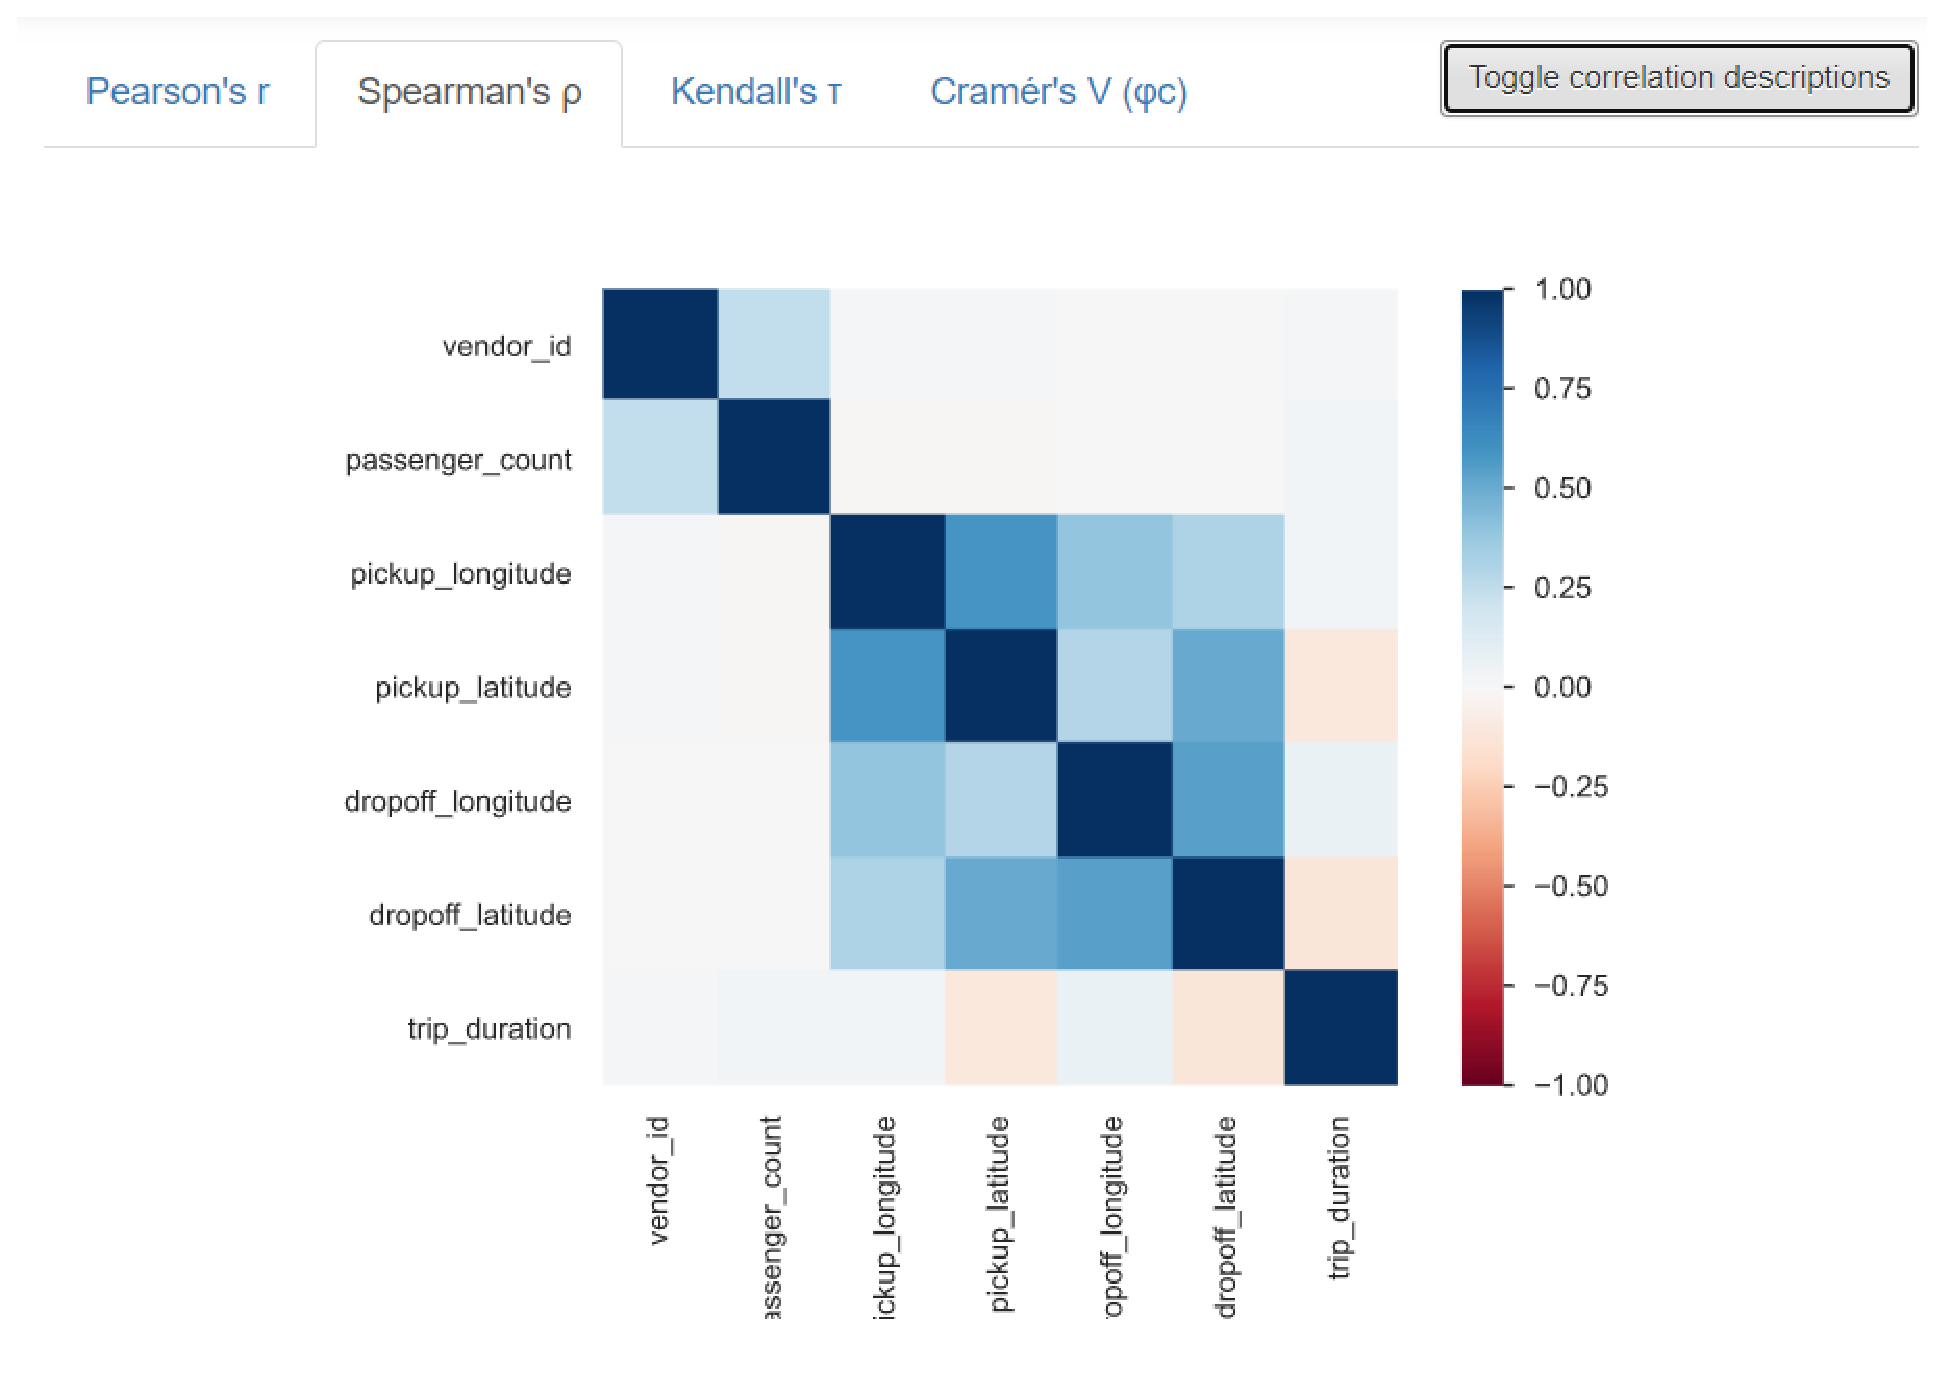
\includegraphics[scale=0.8]{figures/two.eps}
	\end{center}
    \item Duration of taxi trips regard to month,weekday
    \begin{center}
    	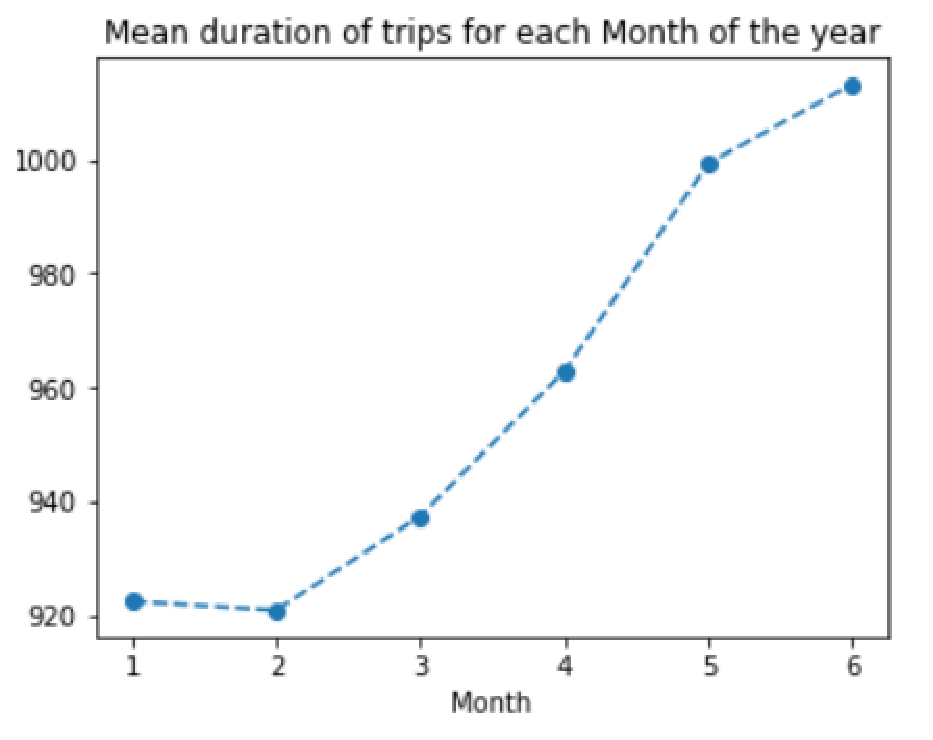
\includegraphics[scale=0.8]{figures/nine.eps}
    	 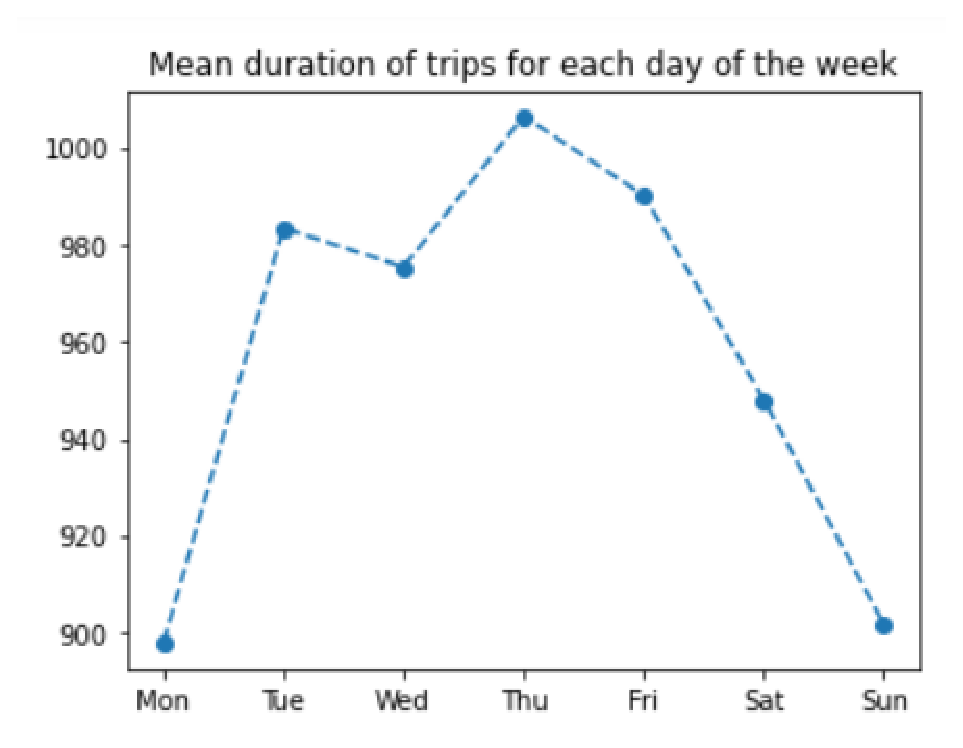
\includegraphics[scale=0.8]{figures/13.eps}
    \end{center}
    \item Pick/Drop locations of taxi trips
    \begin{center}
	 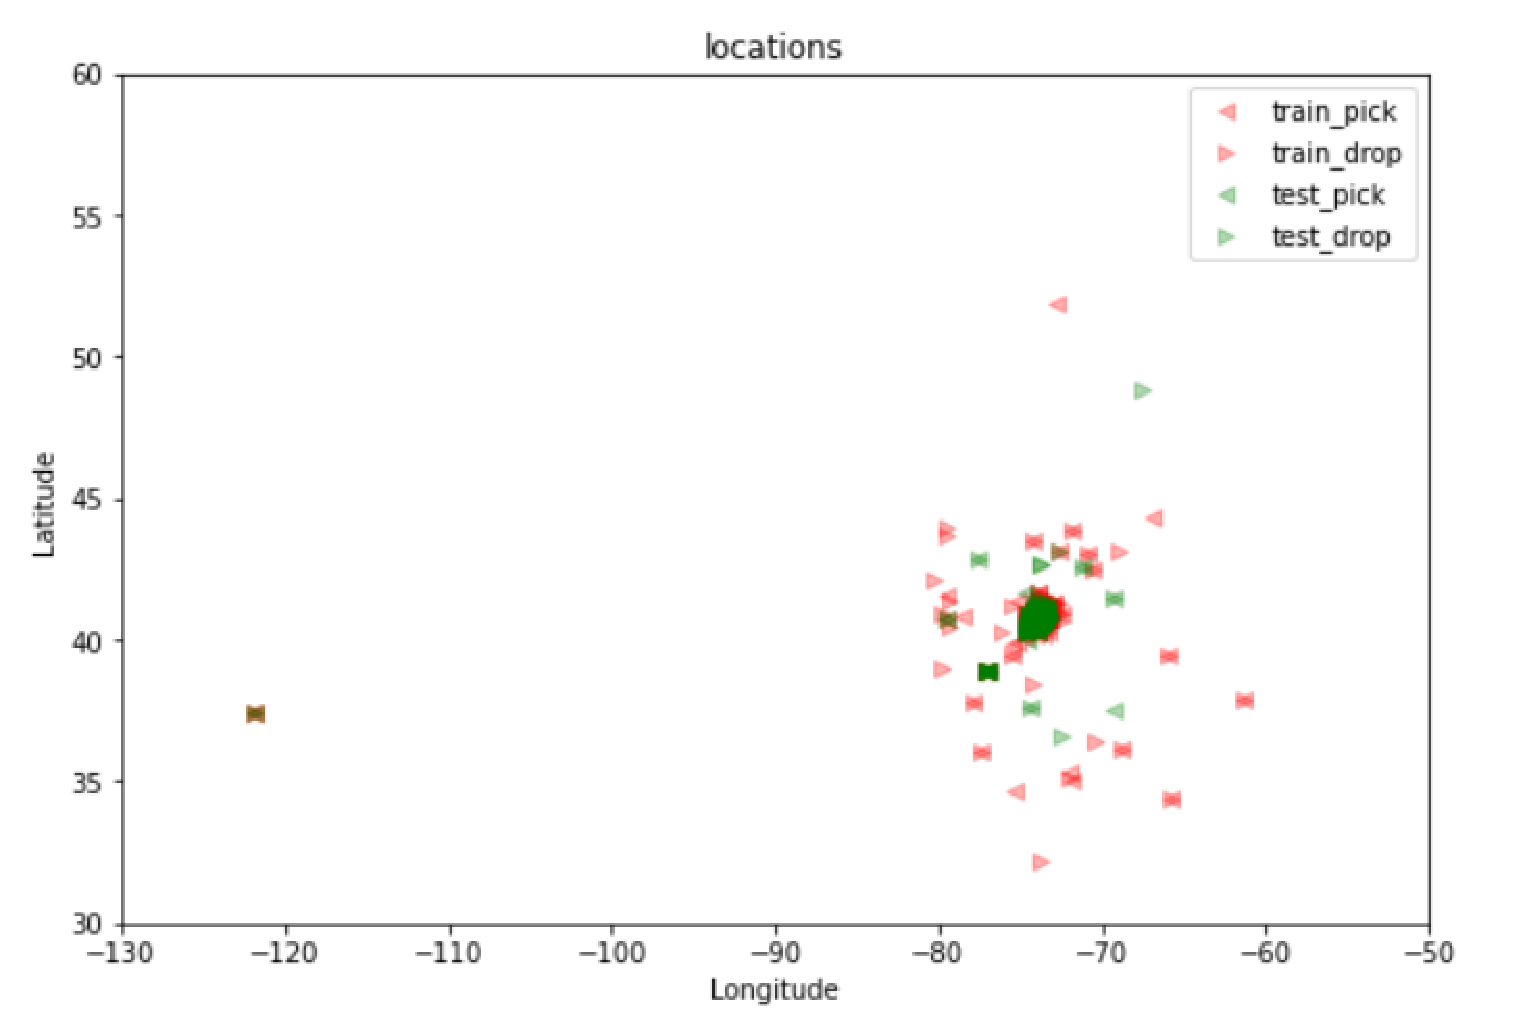
\includegraphics[scale=0.8]{figures/16.eps}
    \end{center}
	\end{itemize}
}
%%%%%%%%%% -------------------------------------------------------------------- %%%%%%%%%%


% SECOND column
\column{0.5}
%Second column with first block's top edge aligned with with previous column's top.

%%%%%%%%%% -------------------------------------------------------------------- %%%%%%%%%%
\block{Feature Selection and Feature Importance}{
	\begin{itemize}
		\item After data Processing,I remove,add and change some attributes.
		\begin{center}
			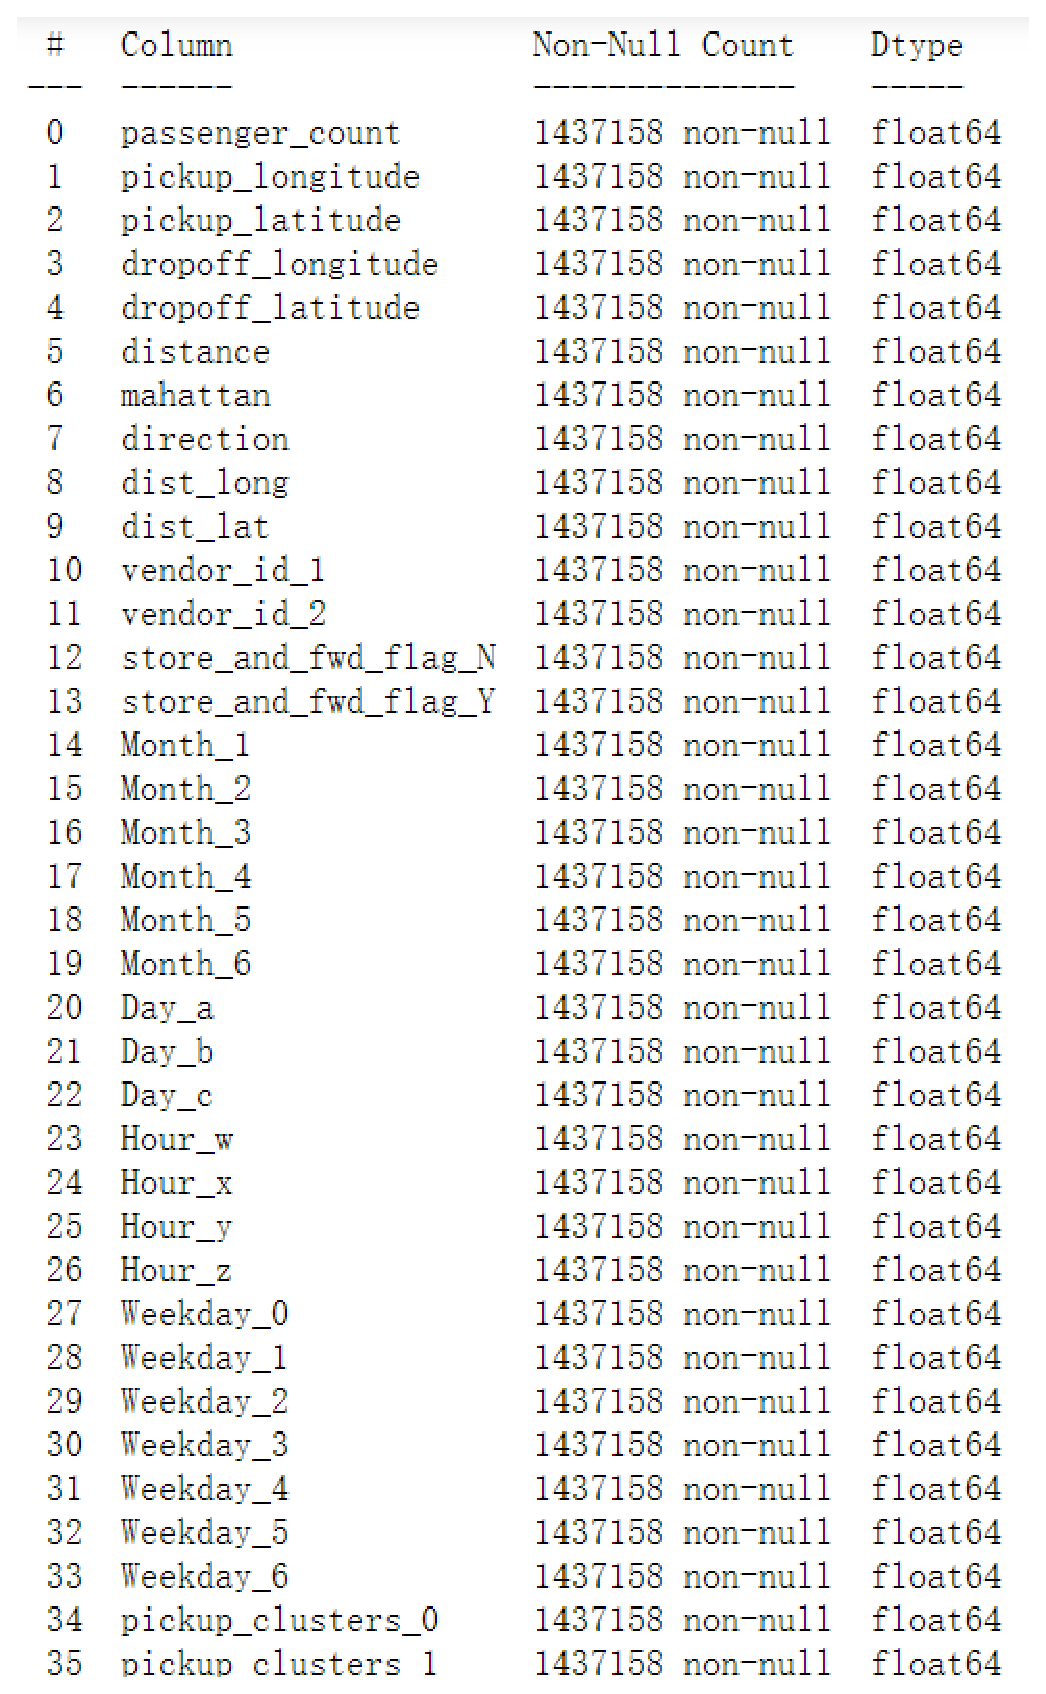
\includegraphics[scale=0.5]{figures/26.eps}
		\end{center}
		\item Feature Importance
		\begin{center}
			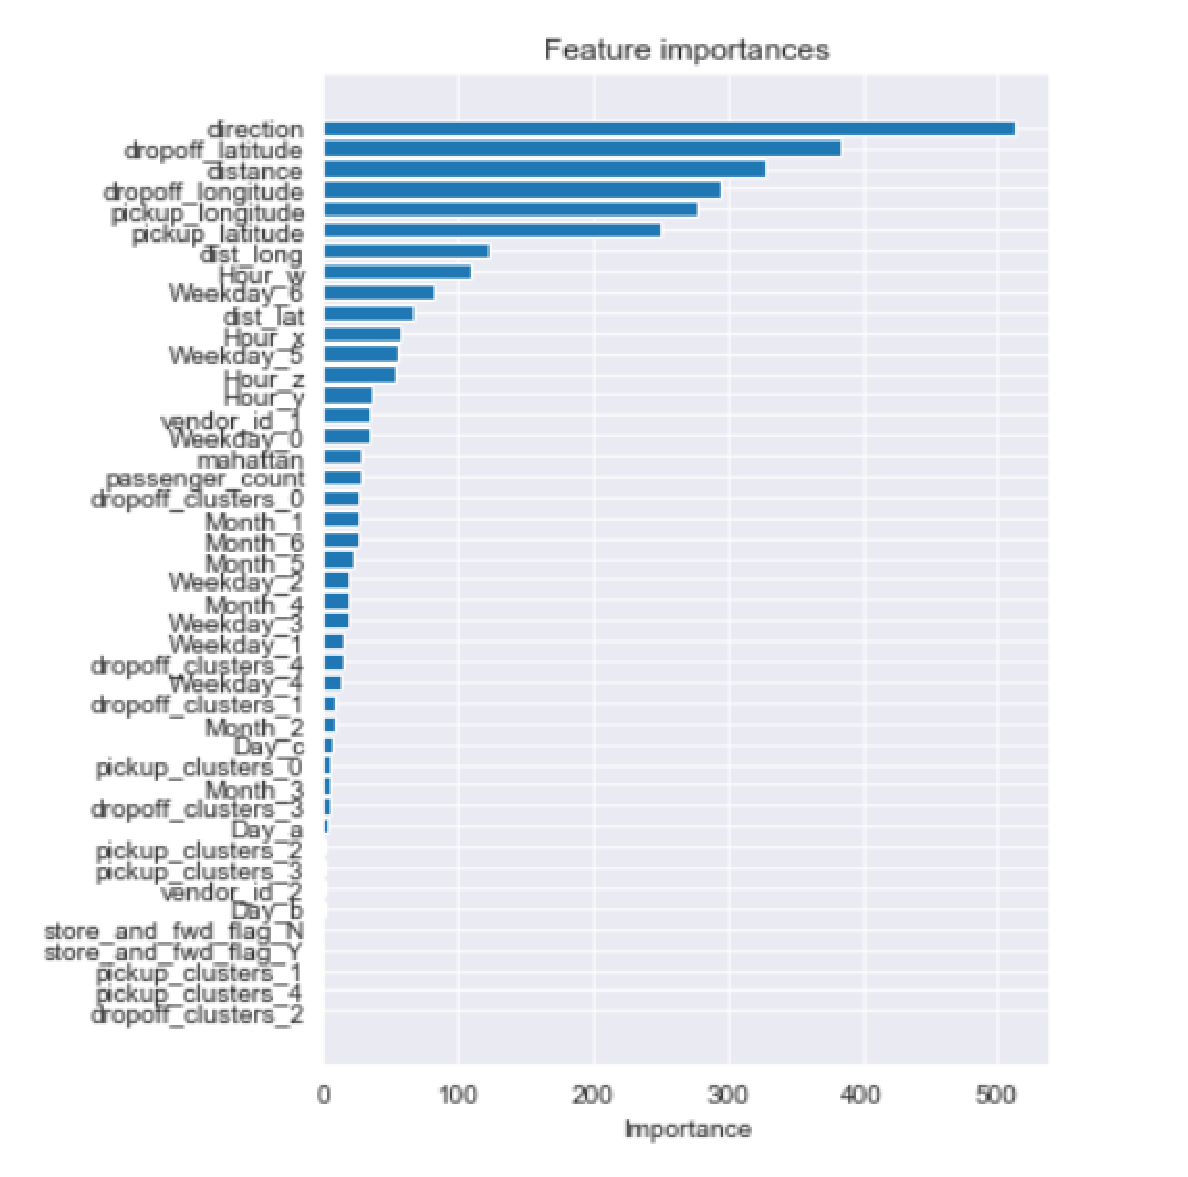
\includegraphics[scale=0.9]{figures/25.eps}
		\end{center}
	\end{itemize}
%	\begin{description}
%		\item
%		Second,
%		based on the \emph{earth move distance},
%		we calculate the outlying degree.
%	\end{description}
%	
%	\begin{tikzfigure}%[Overall architecture of \emph{GOAM} algorithm]
%		\missingfigure[figcolor=white]{Testing figcolor}
%	\end{tikzfigure}
%	where $G_q$ is the query group,
%	$n$ is the number of compare groups,
%	and $h_{k_s}$ is the histogram representation of $G_k$ in the subspace $s$.
%	
%	\begin{description}
%		\item[Outlying Aspects Identification]
%		In this step,
%		based on the value of outlying degree
%		we will identify the group outlying aspects.
%		If a feature's outlying degree is greater than a threshold,
%		the more likely the feature is group outlying aspect.
%		When the dimensionality of features is high,
%		we adopt a stage-wise candidate subspace construction strategy to
%		alleviate the exponential explosion.
%	\end{description}
}
%%%%%%%%%% -------------------------------------------------------------------- %%%%%%%%%%
% Second column - first block


%%%%%%%%%% -------------------------------------------------------------------- %%%%%%%%%%
\block[titleleft]{Model and Result}
{
	\begin{itemize}
		\item Model:Lightgbm and Xgboost
		\item Private score:0.40978
		\item Public score:0.41166
		\begin{center}
			
\includegraphics[scale=0.4]{figures/23.eps}
		\end{center}
		\item Rank:532/1254
	\end{itemize}
%	\begin{description}
%		\item[Synthetic Dataset] contains $10$ groups and $8$ features.
%		Each group consists of $10$ members,
%		and each member has $8$ features.
%	\end{description}
%	\vspace{.5cm}
%	\begin{tabular}{ c | c | c | c }
%		\toprule
%		Method     &  Truth Outlying Aspects    & Identified Aspects & Accuracy      \\
%		\midrule
%		GOAM       &  $\{F_1\}$, $\{F_2F_4\}$   &  $\{F_1\}$, $\{F_2F_4\}$    & 100\%    \\
%		
%		Arithmetic Mean based OAM &  $\{F_1\}$, $\{F_2F_4\}$   &  $\{F_4\}$, $\{F_2\}$    &  0\% \\
%		
%		Median based OAM &  $\{F_1\}$, $\{F_2F_4\}$   &  $\{F_2\}$, $\{F_4\}$    &           0\% \\
%		\bottomrule
%	\end{tabular}
%	\vspace{.2cm}
%	\begin{description}
%		\item
%		It can be observed that the GOAM method can identify the trivial outlying features
%		and non-trivial outlying subspaces correctly and is obvious from the table
%		that the accuracy of GOAM is the best, which is ($100\%$).
%	\end{description}
%	
%	\begin{description}
%		\item[NBA Dataset] was collected from Yahoo Sports
%		website (\url{http://sports.yahoo.com.cn/nba}).
%		The data include all teams from the six divisions,
%		and each player in the team has $12$ features.
%	\end{description}
%	\vspace{.5cm}
%	\begin{tabular}{ c | c | c }
%		\toprule
%		Teams                   & Trivial Outlying Aspects  & NonTrivial Outlying Aspects    \\
%		\toprule
%		Cleveland Cavaliers     & \{3FA\}                   & \{FGA, FT\%\}, \{FGA, FG\%\} \\
%		Orlando Magic           & \{Stl\}                   & None                         \\
%		Milwaukee Bucks         & \{To\}, \{FTA\}           & \{FGA, FTA\}, \{3FA, FTA\}     \\
%		%    Golden State Warriors   & \{FG\%\}                  & \{FT\%, Blk\}, \{FGA, 3PT\%, FTA\}\\
%		%    Utah Jazz               & \{Blk\}                   & \{3FA, 3PT\%\}                    \\
%		New Orleans Pelicans    & \{FT\%\}, \{FTA\}         & \{FTA, Stl\}, \{FTA, To\}          \\
%		\bottomrule
%	\end{tabular}
%	
%	\begin{minipage}{0.5\linewidth}
%		\centering
%		\begin{tikzfigure}
%			\missingfigure[figcolor=white]{Testing figcolor}
%			
%			{\small{New Orleans Pelicans on FT\%}}
%		\end{tikzfigure}%
%	\end{minipage}
%	\hfill
%	\begin{minipage}{0.5\linewidth}
%		\centering
%		\begin{tikzfigure}
%			\missingfigure[figcolor=white]{Testing figcolor}
%			
%			{\small{New Orleans Pelicans on FTA}}
%		\end{tikzfigure}%
%	\end{minipage}
%	\vspace{.2cm}
%	\begin{description}
%		\item
%		\texttt{New Orleans Pelicans} has more players with
%		lower \{free throw percentage\}, \{free throws attempted\}.
%	\end{description}
}
%%%%%%%%%% -------------------------------------------------------------------- %%%%%%%%%%


% Second column - second block
%%%%%%%%%% -------------------------------------------------------------------- %%%%%%%%%%
\block[titlewidthscale=1, bodywidthscale=1]
{Conclusion}
{
	Compare to midterm presentation,My score have greatly imporved from 0.59486 to 0.40978. The reason mainly is more features and more models. In the figure of feature	importance,we can the attribute direction that I added plays a great role. And xgboost model can fit the train data better, but processing speed of lightgbm model is faster.
}
%%%%%%%%%% -------------------------------------------------------------------- %%%%%%%%%%


% Bottomblock
%%%%%%%%%% -------------------------------------------------------------------- %%%%%%%%%%
%\colorlet{notebgcolor}{blue!20}
%\colorlet{notefrcolor}{blue!20}
%\note[targetoffsetx=8cm, targetoffsety=-4cm, angle=30, rotate=15,
%radius=2cm, width=.26\textwidth]{
%	Acknowledgement
%	\begin{itemize}
%		\item
%		International Cooperation Project (Y7Z0511101)
%		of IIE,
%		Chinese Academy of Sciences
%	\end{itemize}
%}

%\note[targetoffsetx=8cm, targetoffsety=-10cm,rotate=0,angle=180,radius=8cm,width=.46\textwidth,innersep=.1cm]{
%Acknowledgement
%}

%\block[titlewidthscale=0.9, bodywidthscale=0.9]
%{Acknowledgement}{
%}
%%%%%%%%%% -------------------------------------------------------------------- %%%%%%%%%%

\end{columns}


%%%%%%%%%% -------------------------------------------------------------------- %%%%%%%%%%
%[titleleft, titleoffsetx=2em, titleoffsety=1em, bodyoffsetx=2em,%
%roundedcorners=10, linewidth=0mm, titlewidthscale=0.7,%
%bodywidthscale=0.9, titlecenter]

%\colorlet{noteframecolor}{blue!20}
\colorlet{notebgcolor}{blue!20}
\colorlet{notefrcolor}{blue!20}
\note[targetoffsetx=-13cm, targetoffsety=-26cm,rotate=0,angle=180,radius=8cm,width=.96\textwidth,innersep=.4cm]
{
\begin{minipage}{0.3\linewidth}
	\centering
	
\includegraphics[width=24cm]{logos/tulip-wordmark.eps}
\end{minipage}
\begin{minipage}{0.7\linewidth}
	{ \centering
		New York City Taxi Trip Duration on Kaggle Competition,
		26/04/2021, Changchun, China
	}
\end{minipage}
}
%%%%%%%%%% -------------------------------------------------------------------- %%%%%%%%%%


\end{document}

%\endinput
%%
%% End of file `tikzposter-template.tex'.